\chapter{Algorytmy oparte na A*}
\label{ch:astar}

Kiedy pojedynczy agent dokonuje znalezienia drogi do wyznaczonego celu, prosty algorytm A* sprawdza się bardzo dobrze. Jednak w przypadku, gdy wiele agentów porusza się w tym samym czasie, to podejście może się nie sprawdzić, powodując wzajemne blokowanie się i zakleszczenie jednostek. Rozwiązaniem tego problemu może być kooperacyjne znajdowanie tras. Roboty będą mogły skutecznie przemieszczać się przez mapę, omijając trasy wyznaczone przez inne jednostki oraz schodząc innym jednostkom z drogi, jeśli to konieczne. \cite{cooppath}

Zagadnienie znajdowania drogi jest ważnym elementem sztucznej inteligencji zaimplementowanej w wielu grach komputerowych. Chociaż klasyczny algorytm A* potrafi doprowadzić pojedynczego agenta do celu, to jednak dla wielu agentów wymagane jest zastosowanie innego podejścia w celu unikania kolizji. Algorytm A* może zostać zaadaptowany do replanowania trasy na żądanie, w przypadku wykrycia kolizji tras (Local Repair A* lub D*). Jednak takie podejście nie jest zadowalające pod wieloma względami. Na trudnych mapach z wieloma wąskimi korytarzami i wieloma agentami może to prowadzić do zakleszczenia agentów w wąskich gardłach lub do cyklicznego zapętlenia ruchu agentów. \cite{cooppath}

\section{Algorytm A*}
A* jest algorytmem heurystycznym służącym do przeszukiwania grafu w celu znalezienia najkrótszej ścieżki. Algorytm ten jest powszechnie stosowany w zagadnieniach sztucznej inteligencji oraz w grach komputerowych \cite{mit_astar}. Jest modyfikacją algorytmu Dijkstry, wprowadza pojęcie funkcji heurystycznej $h(n)$. Wartość funkcji heurystycznej powinna określać przewidywaną drogę do węzła docelowego. W każdym kroku przeszukiwany jest węzeł o najmniejszej wartości funkcji $f(n)$.

\begin{gather}
 	f(n) = g(n) + h(n)
 	\label{eq_astar} 
\end{gather}
 gdzie:

 $g(n)$ - wartość kosztu, dokładna odgległość miedzy węzłem $n$ a węzłęm startowym

 $h(n)$ - heurystyka, przewidywana droga do węzła docelowego

 $n$ - węzeł, wierzchołek przeszukiwanego grafu

Dzięki takiemu podejściu najpierw sprawdzane są najbardziej "obiecujące" rozwiązania, co pozwala szybciej otrzymać rozwiązanie (w przeciwieństwie do algorytmu Dijkstry).
Algorytm kończy działanie w momencie, gdy napotka węzeł będący węzłem docelowym.
Dla każdego odwiedzonego węzła zapamiętywane są wartości $g(n)$, $h(n)$ oraz węzeł będący rodzicem w celu późniejszego odnalezienia drogi powrotnej do węzła startowego po napotkaniu węzła docelowego (por. rys. \ref{fig:image_astar2}).

\begin{figure}[H]
	\centering
	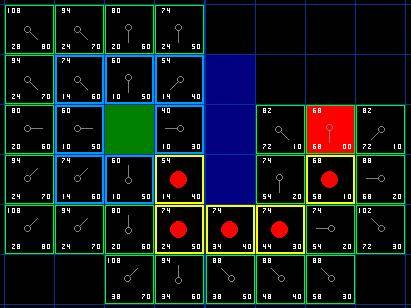
\includegraphics[width=10cm]{img/astar-t7}
	\caption{Przykład działania algorytmu A*. Źródło: \cite{astar2}}
	\label{fig:image_astar2}
\end{figure}

\subsection{Heurystyki}
Od wyboru sposobu obliczania heurystyki zależy czas wykonywania algorytmu oraz optymalność wyznaczonego rozwiązania.
Poniżej przedstawiono najczęściej wykorzystywane heurystyki.

\subsubsection{Heurystyka Euklidesowa}
Dla dwuwymiarowej mapy heurystyka euklidesowa wyraża dokładną odległość między przeszukiwanym węzłem $(x_n, y_n)$ a węzłem docelowym $(x_g, y_g)$:
\begin{gather}
 	h(n) = \sqrt{(x_n - x_g)^2 + (y_n - y_g)^2}
 	\label{eq_astar_heu_euc} 
\end{gather}

\subsubsection{Heurystyka Manhattan}
W przypadku, gdy robot może poruszać się po mapie jedynie poziomo lub pionowo (nie na ukos) wystarczającym przybliżeniem jest metryka Manhattan:
\begin{gather}
 	h(n) = |x_n - x_g| + |y_n - y_g|
 	\label{eq_astar_heu_man} 
\end{gather}

\subsubsection{Heurystyka zerowa}
Przyjęcie heurystyki równej $h(n) = 0$ powoduje, że algorytm A* sprowadza się do algorytmu Dijkstry.

\section{Local Repair A*}
W algorytmie Local Repair A* (LRA*) każdy z agentów znajduje drogę do celu, używając algorytmu A*, ignorując pozostałe roboty oprócz ich obecnych sąsiadów. Roboty zaczynają podążać wyznaczonymi ścieżkami do momentu, aż kolizja z innym robotem jest nieuchronna. Wtedy następuje ponowne przeliczenie drogi pozostałej do przebycia, z uwzględnieniem nowo napotkanej przeszkody.

Możliwe (i całkiem powszechne \cite{cooppath}) jest uzyskanie cykli (tych samych sekwencji ruchów powtarzających się w nieskończoność), dlatego zazwyczaj wprowadzane są pewne modyfikacje, aby rozwiązać ten problem. Jedną z możliwości jest zwiększanie wpływu losowego szumu na wartość heurystyki. Kiedy agenci zachowują się bardziej losowo, prawdopodobne jest, że wydostaną się z problematycznego położenia i spróbują podążać innymi ścieżkami.

Algorytm ten ma jednak sporo poważnych wad, które szczególnie ujawniają się w trudnych środowiskach z dużą liczbą przeszkód. Wydostanie się z zatłoczonego wąskiego gardła może trwać bardzo długo. Prowadzi to również do ponownego przeliczania trasy w prawie każdym kroku. Wciąż możliwe jest również odwiedzanie tych samych lokalizacji w wyniku zapętleń.

\section{Algorytm D*}
D* ({\it Dynamic A* Search}) jest przyrostowym algorytmem przeszukiwania. Jest modyfikacją algorytmu A* pozwalającą na szybsze replanowanie trasy w wyniku zmiany otoczenia (np. zajmowania wolnego pola przez innego robota). Wykorzystywany jest m.in. w nawigacji robota do określonego celu w nieznanym terenie. Początkowo robot planuje drogę na podstawie pewnych założeń (np. nieznany teren nie zawiera przeszkód). Podążając wyznaczoną ścieżką, robot odkrywa rzeczywisty stan mapy i jeśli to konieczne, wykonuje ponowne planowanie trasy na podstawie nowych informacji.
Często wykorzystywaną implementacją (z uwagi na zoptymalizowaną złożoność obliczeniową) jest wariant algorytmu {\it D* Lite} \cite{dstarlite}.

\section{Cooperative A*}
$TODO$

\subsubsection{A* w konfiguracji czaso-przestrzennej}
$TODO$
Algorytm:
\begin{itemize}
	\item Przypisanie priorytetów do poszczególnych robotów
	\item Wykonywanie kroków A* z rozpatrywaniem czasu i przestrzeni - podział otoczenia na siatkę pól, zapisywanie prawdopodobieństwa zajętości pola w danej chwili
\end{itemize}

\section{Hierarchical Cooperative A*}
$TODO$

\section{Windowed Hierarchical Cooperative A*}
$TODO$
